\section*{Tests \& Confidence Intervals}
Want to calculate: $P\left( t_{\alpha / 2, n-p} < \sfrac{\hat \beta_j - \beta_j} {\hat {se}(\hat \beta_j)} < t_{1-\alpha / 2, n-p} \right) = 1 - \alpha$.
$CI = \hat \beta_j \pm \hat se(\hat \beta_j) \cdot t_{1- \alpha / 2, n-p} = \hat \beta_j \pm \hat \sigma \sqrt{x_0^\top (X^\top X)^{-1} x_0} \cdot t_{1- \alpha / 2, n-p}$
\subsection*{Prediction Interval}
For new point $x_0$:
$\hat y_0 = x_0^\top \beta \pm \hat \sigma^2 \sqrt{1 + x_0^\top (X^\top X)^{-1}x_0} \cdot t_{1-\alpha / 2, n-p}$

\textbf{P-Value:} P(obs. a value of the test stat. that is as extreme or more extreme than the one we saw if $H_0$ is true).
If $< \alpha$ then reject $H_0$.

% Too lazy to draw this in LaTeX ;)
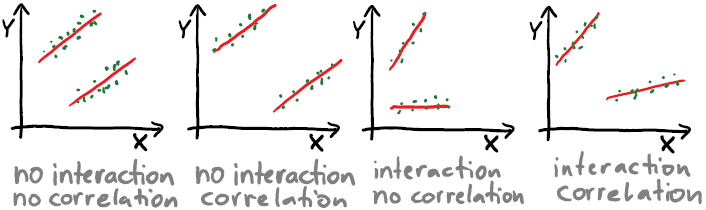
\includegraphics[width=0.7\linewidth]{img/interaction.PNG}

\subsection*{Bias Variance Trade-Off}
Expected Test MSE at $x_0$: $\Ex[(y_0 - \hat f(x_0)^2] = \text{Bias}^2 (\hat f(x_0)) + \text{Var}(\hat f(x_0)) + \sigma^2$, where $\text{Bias}^2(\hat f(x_0)) = (f(x_0)-\Ex[\hat f(x_0)])^2$, $Bias = \Ex[\hat f(x_0)] - f(x_0)$ (see code).

\textbf{Notation}
$Y_i=f(X_i)+\epsilon_i$, where $\epsilon_i$ iid, $\Ex[\epsilon_i]=0$, $\Var(\epsilon_i)=\sigma^2$. $f$ is arbitrary fixed unknown function. Consider estimator $\hat f$ trained/fitted on $(x_1,y_1),...,(x_n,y_n)$. Then Training MSE: $\tfrac{1}{n} \sum_{i=1}^n (y_i-\hat f(x_i))^2$. Test MSE on new sample $(\tilde x_1, \tilde y_1),...,(\tilde x_m, \tilde y_m)$: $\tfrac{1}{m}\sum_{i=1}^m (\tilde y_i-\hat f(\tilde x_i))^2$.

\textbf{Trade off}
Consider new pair $(x_0,y_0)$: Then $\Ex[(y_0-\hat f(x_0))^2]=(f(x_0)-\Ex[\hat f(x_0)])^2+\Var(\hat f(x_0))+\Var(\epsilon)=(\textup{Bias}(\hat f(x_0)))^2+\Var(\hat f(x_0))+{\sigma^2}$, $\sigma^2$ irreducable error, where Exp. is over different training sets.

\begin{codebox}{r}{Confidence Intervals \& p-value}
  # P-value: variant 1, 1 sided, H0: <= 6
  res <-  replicate(nsimul, simulateSomething())
  pval.1 <- (1+sum(res.1 <= 6))/(nsimul+1)
  # P-value: variant 2
  pval.2 <- 2*pt(qt(1-alpha/2,n-p), df=n-p, lower=FALSE)
  confint(fit) # Automatic CI.
  # Manual CI (for intercept):
  se.intercept <- summary(fit)$coef[1,2]
    coef(fit)[1] - qt(.975, n-2)*se.intercept
    coef(fit)[1] + qt(.975, n-2)*se.intercept
    # Predict value and C.I. (c for $\Ex[Y_0]$, p for $Y_0$):
    # Automatic Prediction CI
    predict(fit,newdata=data.frame(name=5), level=.95, interval="p")
    # Automatic CI
    predict(fit,newdata=data.frame(name=5), level=.95, interval="c")
    # Manual Prediction CI
    fitted <- fit$coef[1] + fit$coef[2]*x0
    quant <- qt(.975,n-2) # Quantile of t distribution
    sigma.hat <- sqrt(sum((fit$resid)^2/(n-2)))
  X <- as.matrix(cbind(1,thuesen[,1]))
  XtXi <- solve(t(X) %*% X) # (X^T X)^{-1}
  X00 <- as.matrix(c(1,x0), nrow=2)
  se <- sigma.hat * sqrt(t(X00) %*% XtXi %*% x00)
  lower <- fitted - quant * se
  upper <- fitted + quant * se
  # Bias Variance Trade-Off of a Method
  Bias <- mean(EstimateUsingCV) - TrueValueSimulated
  MSE <- Bias^2 + var(EstimateUsingCV)
\end{codebox}
